\documentclass{beamer}

\usetheme[numbering=fraction, progressbar=foot]{metropolis}

\usepackage{appendixnumberbeamer}
\usepackage[backend=biber,style=apa]{biblatex}
\usepackage{animate}
\usepackage{booktabs}
\usepackage{multirow}

\definecolor{imperial_blue}{RGB}{23, 63, 140}
\setbeamercolor{alerted text}{fg=imperial_blue}
\setbeamercolor{frametitle}{bg=imperial_blue}

\addbibresource{references.bib}

\title{SMC-Guided Diffusion for General Optimisation}
\date{\today}
\author{Brendan Dowling, Dr O. Deniz Akyildiz}
\institute{Imperial College London}
\titlegraphic{\hfill
\includegraphics[height=0.4cm]{assets/imperial_logo.pdf}}

\begin{document}

    \maketitle

    \begin{frame}{Table of contents}
        \setbeamertemplate{section in toc}[sections numbered]
        \tableofcontents[hideallsubsections]
    \end{frame}

    \section{Introduction}
    \begin{frame}{First Frame}
        Hello, world! \textcite{andersonReversetimeDiffusionEquation1982,hoDenoisingDiffusionProbabilistic2020,douDiffusionPosteriorSampling2023,akyildizParallelSequentialMonte2020,delmoralCentralLimitTheorems2011}
    \end{frame}

    \section{Background}

    \begin{frame}{Annealing}
        Text
    \end{frame}

    \begin{frame}{Inverse Problems}
        Text
    \end{frame}

    \begin{frame}{Diffusion Models}
        Text
    \end{frame}

    \begin{frame}{Sequential Monte Carlo}
        Text
    \end{frame}

    \section{\texttt{SMCDiffOpt}}

    \begin{frame}{Heuritic Motivation}
        Text
    \end{frame}

    \begin{frame}{Algorithm}
        Text
    \end{frame}

    \begin{frame}{Geometric Interpretation}
        Text
    \end{frame}

    \begin{frame}{Appyling to Inverse Problems}
        Text
    \end{frame}

    \section{Experimental Results}

    \begin{frame}{GMM Experiment --- Setup}
        Consider a Gaussian mixture model (GMM), $p_{\text{data}}$, with 25 equally weighted
        ($\omega_{i,j} \propto 1$) $d_x$-dimensional Gaussian random variables with means
        $\mathbf{\mu}_{i,j} := (8i, 8j, \dots, 8i, 8j) \in \mathbb{R}^{d_x}$
        for $(i, j)\in \{-2, \ldots, 2\}^2$ and unit variance.
        We generate some $d_y$-dimensional measurement, $\mathbf{y}$, according to the following process:
        \begin{itemize}
            \item Draw $\tilde{A} \sim \mathcal{N}(0, 1)^{d_y \times d_x} \in \mathbb{R}^{d_y \times d_x}$
            and compute its SVD decomposition, $USV^\top$.
            \item Sample $s_{i,j} \sim \mathcal{U}[0,1]$ for $(i,j) \in \{-2, \dots, 2\}^2$.
            \item Set $A := U\, diag(\{s_{i,j}\})\, V^\top$.
            \item Draw $\mathbf{x}_* \sim p_{\text{data}}$ and set $\mathbf{y} := A\mathbf{x}_* + \sigma_y\epsilon,\ \epsilon \sim \mathcal{N}(\mathbf{0}_{d_y}, \mathrm{I}_{d_y})$.
        \end{itemize}
        
        The goal of the inverse problem is to take $\mathbf{y}$ (with $A$ and $\sigma_y$ known), and use
        it to infer $\mathbf{x}_*$. We consider $d_y < d_x$, making the problem ill-posed.
    \end{frame}

    \begin{frame}{GMM Experiment --- Setup Visualised}
        \centering
        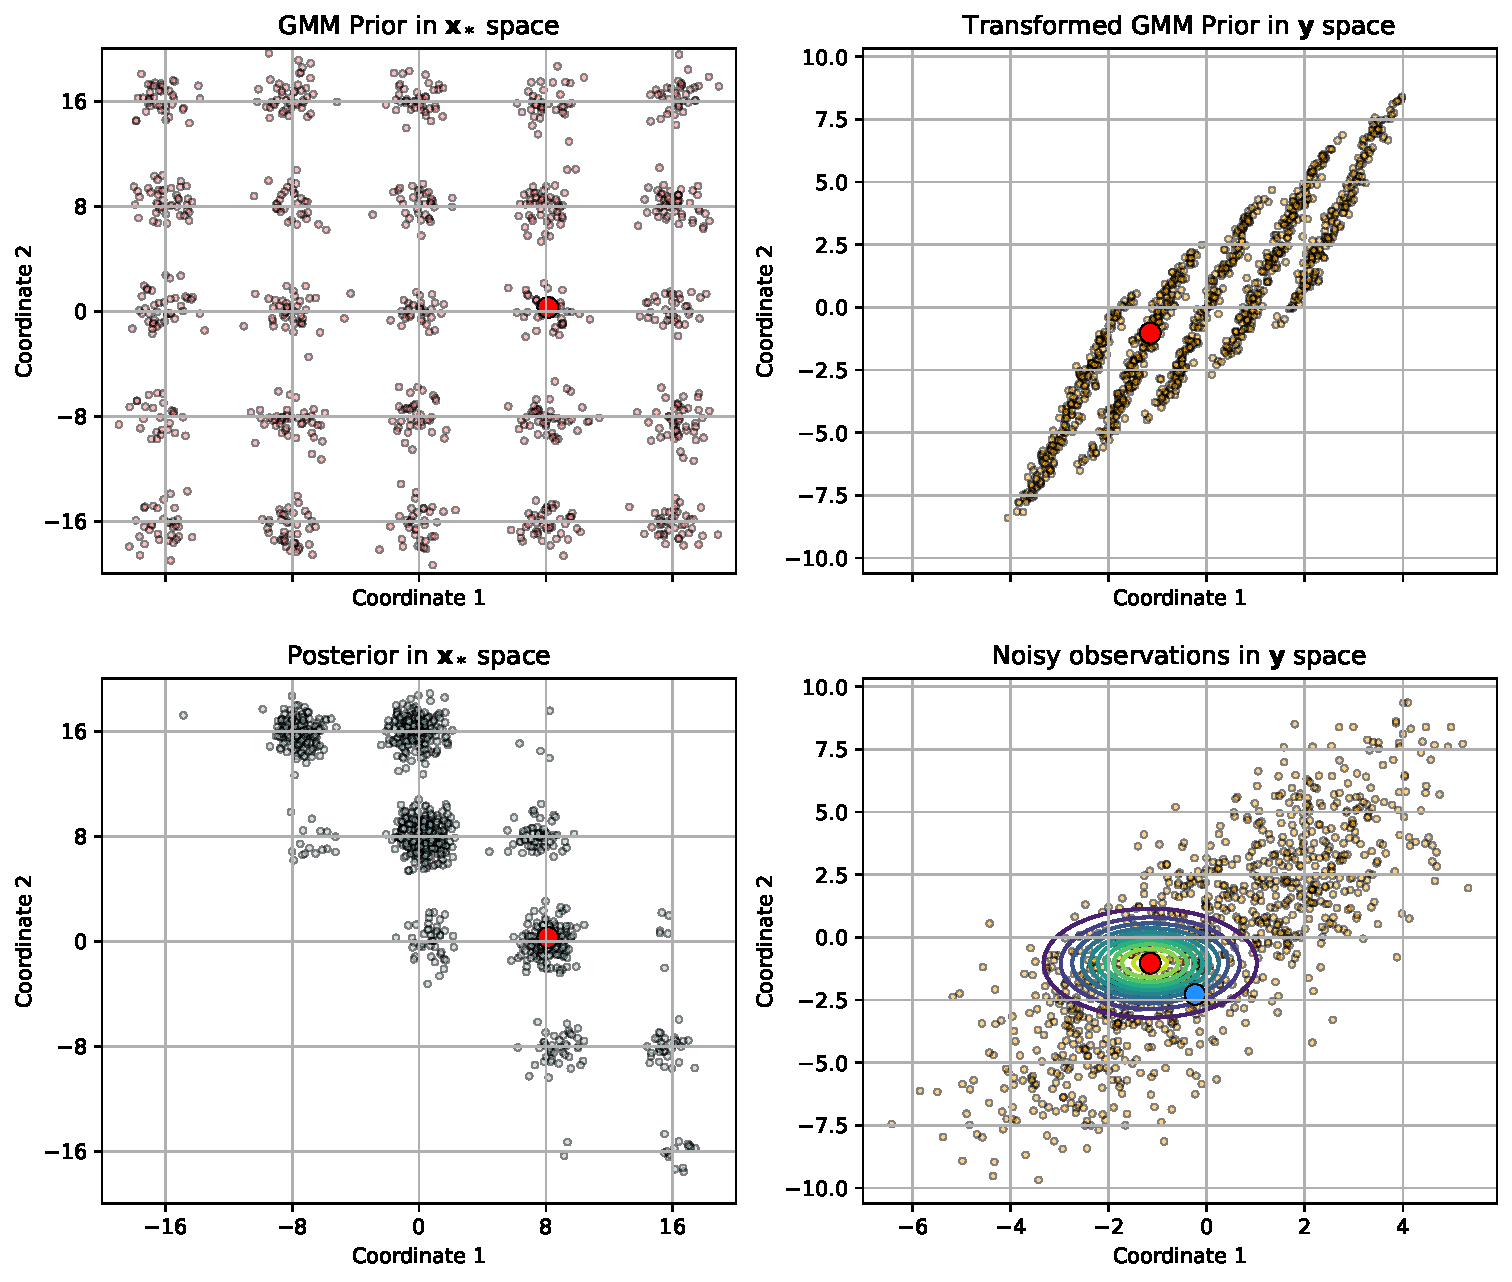
\includegraphics[width=0.98\textwidth]{assets/gmm-measurement-system.pdf}
    \end{frame}

    \begin{frame}{GMM Experiment --- Prior Model and TMPD Guidance}
        \centering
        % \animategraphics[loop,width=5cm]{25}{assets/gmm-prior/gmm-prior-}{0}{200}
        % \animategraphics[loop,width=5cm]{25}{assets/gmm-posterior-vjp_guidance/gmm-posterior-vjp_guidance-}{0}{200}
    \end{frame}

    \begin{frame}{GMM Experiment --- \texttt{SMCDiffOpt}}
        \centering
        % \animategraphics[loop,width=5cm]{25}{assets/gmm-prior/gmm-prior-}{0}{200}
        % \animategraphics[loop,width=5cm]{25}{assets/gmm-posterior-smc_diff_opt/gmm-posterior-smc_diff_opt-}{0}{200}
    \end{frame}

    \begin{frame}{GMM Experiment --- Performance Comparison}
        \begin{table}[t]
            \centering
            \resizebox{\textwidth}{!}{
            \begin{tabular}{llllll}
                \toprule
                $d_x$ & $d_y$ & SMCDiffOpt & DPS & $\Pi$IGD & TMPD \\
                \midrule
                \multirow[t]{3}{*}{8} & 1 & \textbf{1.35 ± 1.0} & 8.18 ± 7.5 & 3.16 ± 2.72 & 3.31 ± 2.86 \\
                 & 2 & \textbf{0.55 ± 0.43} & 2.72 ± 2.62 & 0.94 ± 0.89 & 1.34 ± 1.25 \\
                 & 4 & 0.19 ± 0.09 & 0.95 ± 0.9 & \textbf{0.09 ± 0.03} & 0.37 ± 0.33 \\
                \cline{1-6}
                \multirow[t]{3}{*}{80} & 1 & \textbf{1.65 ± 1.41} & 5.03 ± 4.63 & 3.08 ± 2.71 & 2.42 ± 1.71 \\
                 & 2 & \textbf{1.19 ± 1.07} & 3.14 ± 3.02 & 1.68 ± 1.62 & 1.35 ± 1.22 \\
                 & 4 & 1.11 ± 0.93 & 1.32 ± 1.21 & \textbf{0.84 ± 0.79} & 1.14 ± 0.9 \\
                \cline{1-6}
                \bottomrule
            \end{tabular}
            }
            \caption{Sliced-Wasserstein distances of samples from particle samples.}
        \end{table}
    \end{frame}

    \begin{frame}{Branin Experiment --- Setup}
        Consider optimising the Branin function as an objective over
        some constrained region (the data manifold) as detailed in
        \textcite{kongDiffusionModelsConstrained2024}. The Branin function is defined by
        \begin{equation*}
            f(x_1, x_2) = a(x_2 - bx_1^2 + cx_1 - r)^2 + s(1-t)\cos(x_1) + s
        \end{equation*}
        where $a=1$, $b = \frac{5.1}{4\pi^2}$, $c=\frac{5}{\pi}$, $r=6$, $s=10$, $t=\frac{1}{8\pi}$.
        It has three global minima located at $(-\pi, 12.275)$, $(\pi, 2.275)$ and $(9.42478, 2.475)$,
        with a value of $0.397887$. We consider some uniform prior sampling distribution, $p_{\text{data}}$,
        over an ellipse region centred at $(-0.2, 7.5)$ with semi-axis lengths $(3.6, 8)$, tilted
        $25^\circ$. This region covers two of the global minima.
    \end{frame}

    \begin{frame}{Branin Experiment --- Pitfalls of Gradient Optimisation}
        \centering
        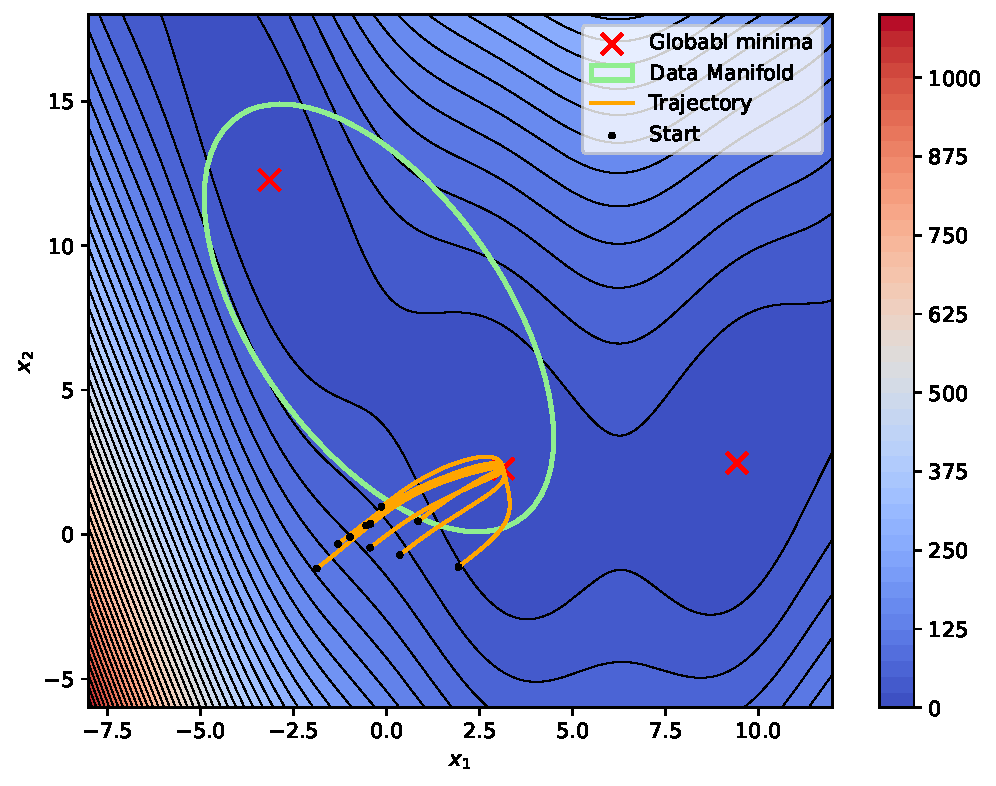
\includegraphics[width=\textwidth]{assets/adam_branin.pdf}
    \end{frame}

    \begin{frame}{Branin Experiment --- Pitfalls of Gradient Optimisation II}
        \centering
        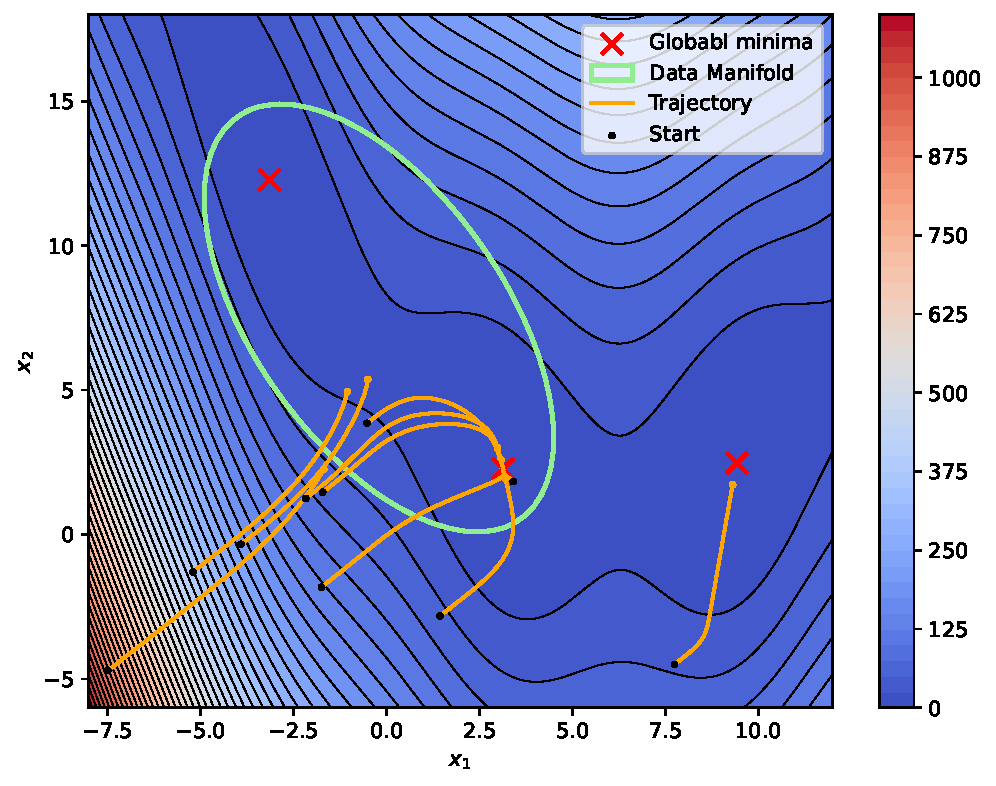
\includegraphics[width=\textwidth]{assets/adam_larger_branin.pdf}
    \end{frame}

    \begin{frame}{Branin Experiment --- \texttt{SMCDiffOpt}}

    \end{frame}

    \begin{frame}{Black-Box Experiment --- Motivation}
        Text
    \end{frame}

    \begin{frame}{Black-Box Experiment --- Setup}
        Text
    \end{frame}

    \begin{frame}{Black-Box Experiment --- Real Sample}
        \centering
        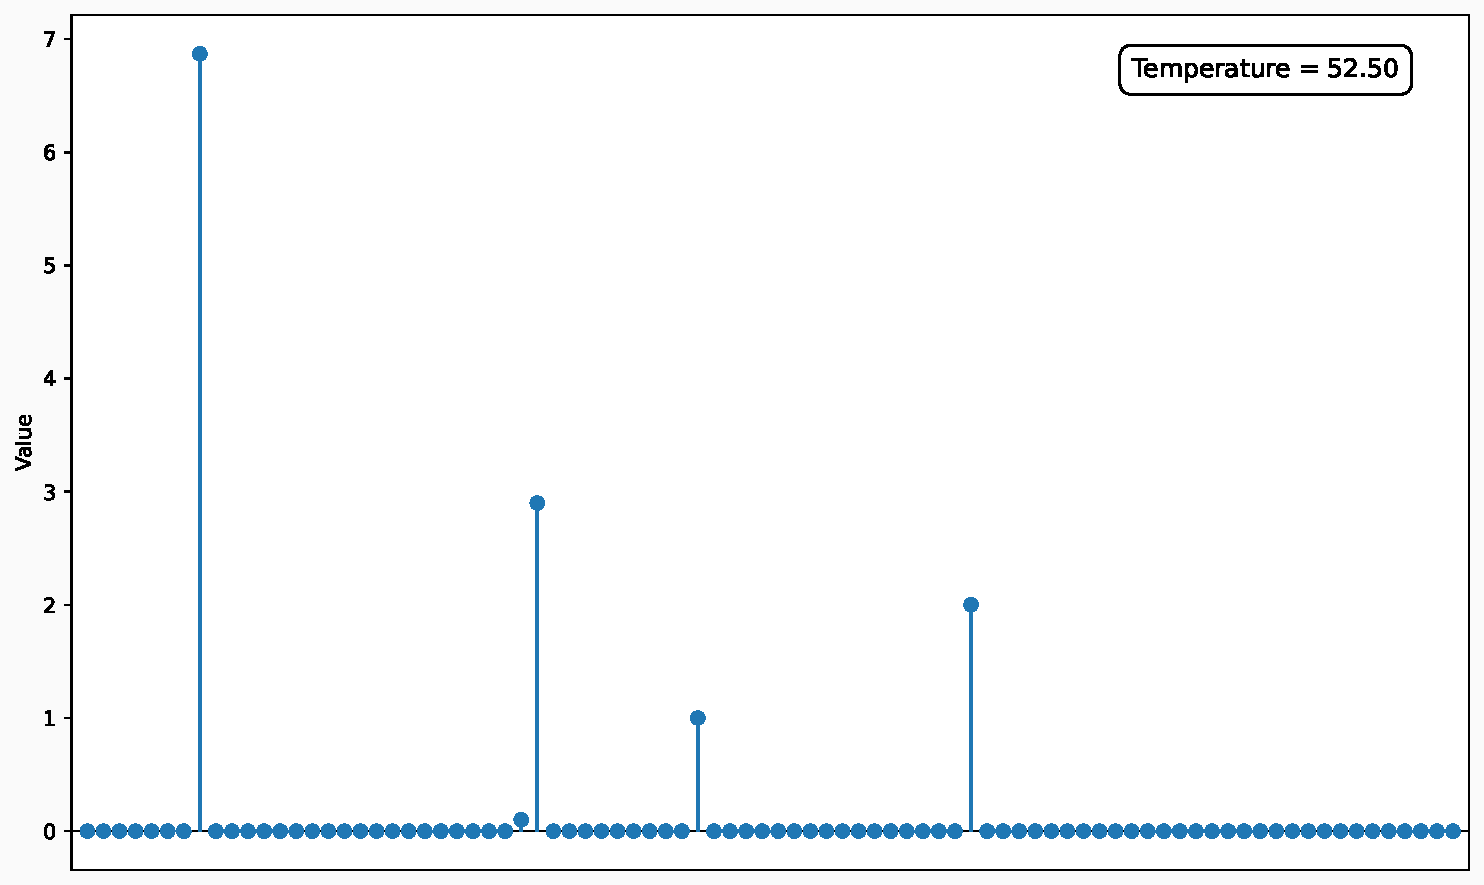
\includegraphics[width=1\textwidth]{assets/bb-real-sample.pdf}
    \end{frame}

    \begin{frame}{Black-Box Experiment --- Generated Sample}
        \centering
        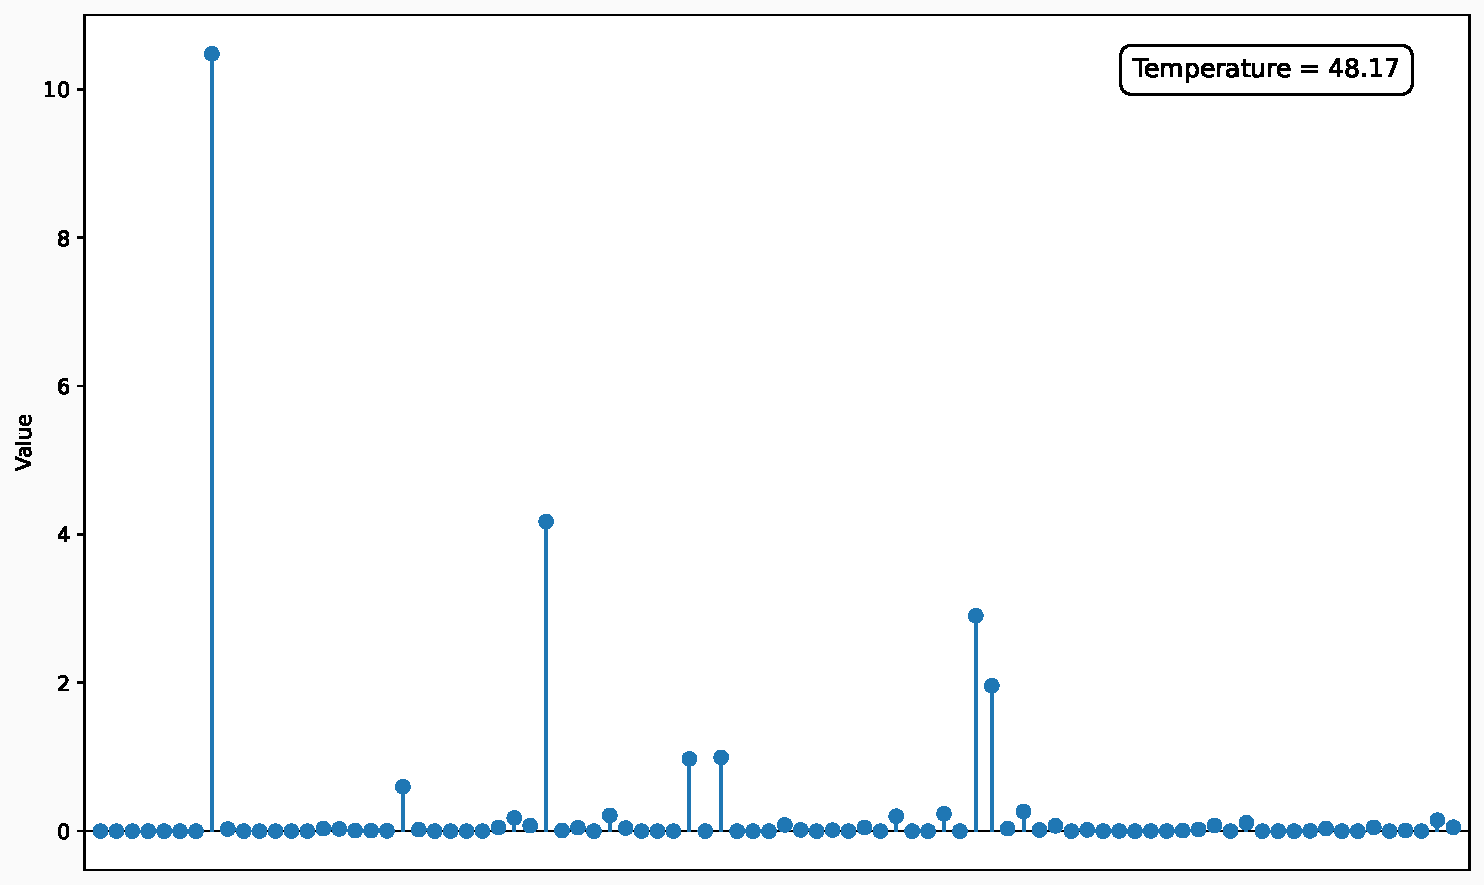
\includegraphics[width=1\textwidth]{assets/bb-unconditional-sample.pdf}
    \end{frame}

    \begin{frame}{Black-Box Experiment --- Optimised Sample}
        \centering
        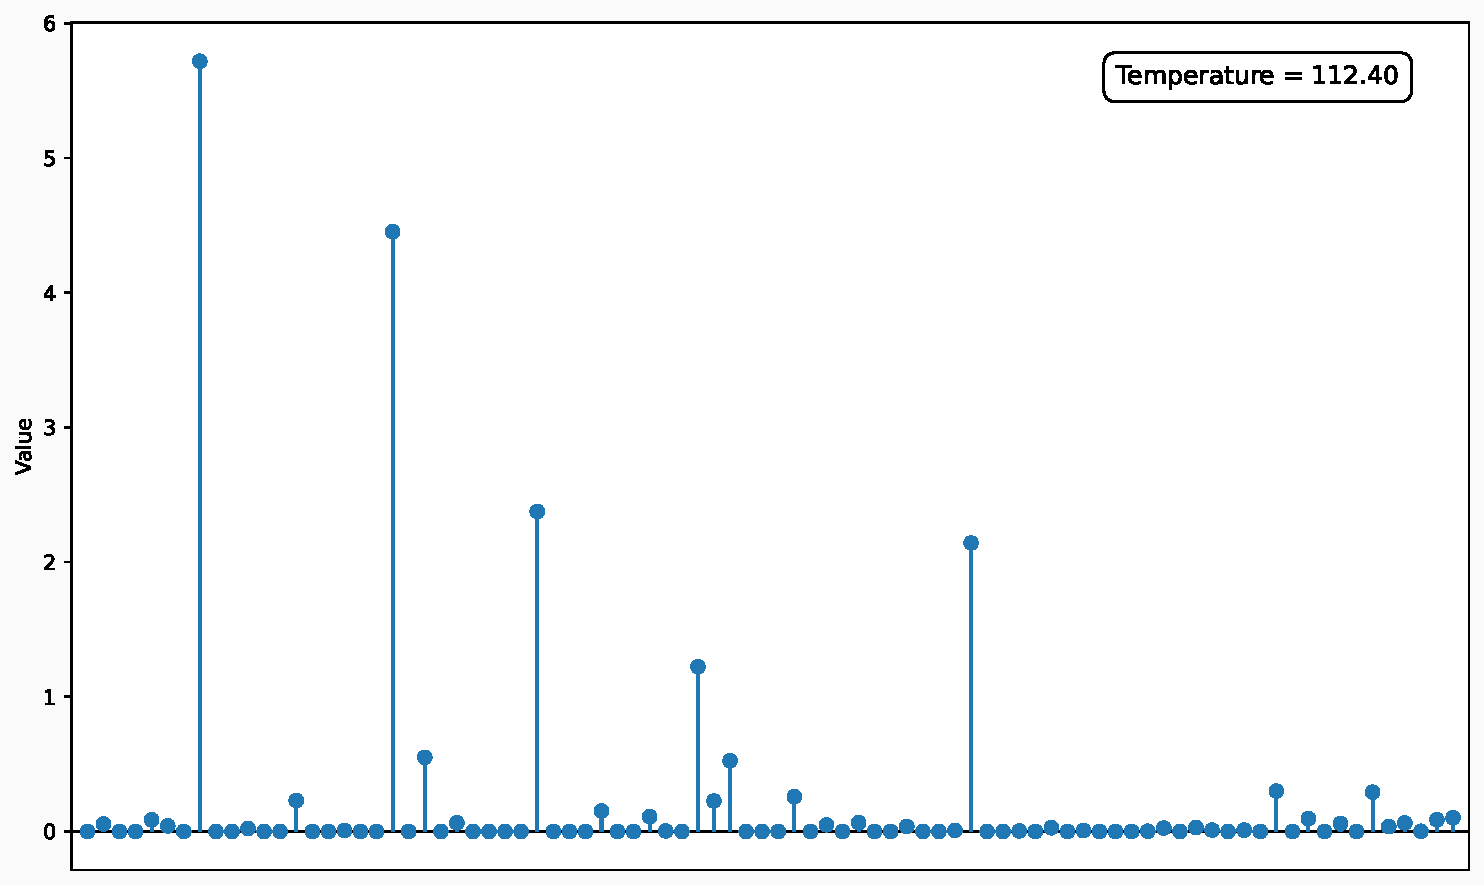
\includegraphics[width=1\textwidth]{assets/bb-optimised-sample.pdf}
    \end{frame}

    \begin{frame}{Black-Box Experiment --- Performance Comparison}
        \begin{table}[t]
            \centering
            \resizebox{\textwidth}{!}{
            \begin{tabular}{llllllll}
                \toprule
                CbAS & CMA-ES & Gradient Ascent & MINs & REINFORCE & DDOM & DiffOpt & \textbf{SMCDiffOpt} \\
                \midrule
                0.433 ± 0.027 & 0.474 ± 0.021 & 0.510 ± 0.009 & 0.473 ± 0.003 & 0.483 ± 0.015 & 0.560 ± 0.044 & 0.614 ± 0.029 & \textbf{0.644 ± 0.024} \\
                \bottomrule
            \end{tabular}
            }
            \caption{Normalised scores for SuperConductor experiment.}
        \end{table}
        \begin{table}[t]
            \centering
            \resizebox{\textwidth}{!}{
            \begin{tabular}{llllllll}
                \toprule
                CbAS & CMA-ES & Gradient Ascent & MINs & REINFORCE & DDOM & DiffOpt & \textbf{SMCDiffOpt} \\
                \midrule
                80.082 ± 4.933 & 87.774 ± 3.965 & 94.414 ± 1.719 & 87.483 ± 0.481 & 89.351 ± 2.708 & 103.600 ± 8.139 & 113.545 ± 5.322 & \textbf{119.059 ± 4.497} \\
                \bottomrule
            \end{tabular}
            }
            \caption{Raw scores for SuperConductor experiment.}
        \end{table}
    \end{frame}

    \section{Conclusion}

    \begin{frame}{Future Work}
        Text
    \end{frame}

    \begin{frame}{Final Remarks}
        Text
    \end{frame}

    % \begin{frame}{Animation}
    %     \centering
    %     \animategraphics[loop,width=5cm]{25}{assets/gmm-prior/gmm-prior-}{0}{200}
    %     \animategraphics[loop,width=5cm]{25}{assets/gmm-posterior-smc_diff_opt/gmm-posterior-smc_diff_opt-}{0}{200}
    % \end{frame}

    {
    \setbeamercolor{palette primary}{bg=imperial_blue}
    \begin{frame}[standout]
        Thank you!
    \end{frame}
    }

    \appendix

    \begin{frame}[allowframebreaks]{References}
        \printbibliography[heading=none]
    \end{frame}

\end{document}
